\documentclass{iopjournal}
\usepackage{graphicx}
\usepackage{booktabs}
\usepackage{siunitx}
\usepackage{amsmath}

\begin{document}

\articletype{Research Article}
\title{LoMI-SSL: A Standardized Few-Shot Motor Imagery Calibration Benchmark with Compact Self-Supervised Encoders}

\author{S. Khresth$^{1,*}$}
\affil{$^1$School of Computing, University of Leeds, Leeds, United Kingdom}
\affil{$^*$Author to whom any correspondence should be addressed.}
\email{shkry.research@outlook.com}
\keywords{motor imagery, brain-computer interface, self-supervised learning, few-shot learning, EEG decoding}

\begin{abstract}
Motor imagery (MI) brain-computer interfaces require extensive per-user calibration (typically 50--200 labeled trials), limiting clinical deployment. We introduce \textbf{LoMI-SSL}, the first standardized benchmark for low-shot MI calibration using self-supervised pretraining. 

Protocol: session-wise splits across BNCI2014-001 (n=9 subjects) and PhysionetMI (n=20 subjects), fixed budgets $\{5,10,20,50\}$ trials/class $\times$ 5 repeats with deterministic seeds. Baselines include CSP+LDA (\textbf{58.8\%@5-shot}), EEGNet-from-scratch (50.2\%), masked reconstruction SSL (\textbf{63.9\%}), and physiology-aware $\mu$/$\beta$ SSL (64.2\%).

SSL methods outperform deep-from-scratch training (+13.7\% BNCI2014-001, +7.2\% PhysionetMI) but exhibit dataset dependence and fail to generalize in frozen-probe settings. Cross-dataset transfer (BNCI$\rightarrow$PhysionetMI) reveals substantial generalization gaps. We release a complete reproducible pipeline with MOABB integration, exact seeds, and deployment metrics (ONNX CPU inference \SI{0.358}{\milli\second}). LoMI-SSL enables rigorous evaluation of SSL methods for practical BCI calibration.
\end{abstract}

\section{Introduction}

Motor imagery (MI) brain-computer interfaces (BCIs) enable direct neural control of external devices but face a critical calibration bottleneck: 50--200 labeled trials per user are typically required for reliable decoding \cite{lotte2018review}. This calibration burden limits clinical deployment, particularly for patients with severe motor impairments who cannot provide extensive training data.

Recent self-supervised learning (SSL) methods show promise for EEG representation learning \cite{banville2021self}, but lack standardized few-shot evaluation protocols. Existing MI benchmarks use within-session cross-validation, ignoring the cross-session generalization required for real-world deployment \cite{vandecappelle2022moabb}.

\textbf{LoMI-SSL} fills this gap with:
\begin{itemize}
\item First standardized few-shot MI calibration protocol (session-wise splits, $\{5,10,20,50\}$ trials/class $\times$ 5 repeats)
\item Multi-dataset evaluation (BNCI2014-001 + PhysionetMI, n=29 total)
\item Baseline suite: CSP+LDA, EEGNet-from-scratch, masked reconstruction SSL, physiology-aware $\mu$/$\beta$ SSL
\item Cross-dataset transfer benchmark (BNCI$\rightarrow$PhysionetMI)
\item Deployment metrics (ONNX CPU \SI{0.358}{\milli\second}, RTX 4050 validated)
\end{itemize}

\section{LoMI-SSL Protocol}

\subsection{Datasets and Splits}

\textbf{BNCI2014-001} \cite{tangermann2012benchmark}: 9 subjects, 22-channel EEG, 4-class MI (left/right hand/foot/tongue), 250\,Hz. Session split: 0train $\rightarrow$ 1test.

\textbf{PhysionetMI} \cite{goldberger2000physiobank}: 20 subjects, 64-channel EEG, 2-class fist MI (left/right), 160\,Hz. Run-based split: runs 0/1 $\rightarrow$ run 2 (leakage-free equivalent).

\subsection{Few-Shot Evaluation}

For each subject and budget $k \in \{5,10,20,50\}$ trials/class:
\begin{enumerate}
\item Sample $k$ trials/class from training session (5 repeats, seeds 42--46)
\item Train decoder on $2k$ total calibration trials
\item Evaluate on full held-out test session
\item Report mean$\pm$std across repeats
\end{enumerate}

Total calibration: 20/40/80/200 trials across 2 classes (10/20/40/100 min sessions).

\subsection{Preprocessing}

\textbf{LeftRightImagery} paradigm (MOABB): 8--32\,Hz bandpass, 128\,Hz downsampling, CSP-compatible preprocessing.

\subsection{Baselines}

\begin{table}
\centering
\caption{Model specifications}
\label{tab:models}
\begin{tabular}{ll}
\toprule
Method & Parameters \\
\midrule
CSP+LDA & scikit-learn CSP($n_\text{comp}=4$)+LDA \\
EEGNet-from-scratch & Braindecode EEGNetv4, Adam 1e-3, 80 epochs \\
MaskedSSL & Conv1D encoder (48k params), masked reconstruction \\
$\mu$/$\beta$ SSL & Same encoder, NT-Xent on 8--30\,Hz vs non-MI bands \\
\bottomrule
\end{tabular}
\end{table}

\textbf{Evaluation modes}: (1) frozen encoder + linear probe, (2) full fine-tuning.

\section{Results}

Table~\ref{tab:leaderboard} shows the 5-shot leaderboard. SSL methods substantially outperform EEGNet-from-scratch (+13.7\% BNCI, +7.2\% PhysionetMI) and match/exceed CSP on clean data.

\begin{table}
\centering
\caption{LoMI-SSL 5-shot leaderboard (mean accuracy \%). Bold = best per dataset.}
\label{tab:leaderboard}
\begin{tabular}{lcccc}
\toprule
Dataset & CSP+LDA & EEGNet & MaskedSSL-FT & $\mu$/$\beta$ SSL-FT \\
\midrule
BNCI2014-001 & 58.8 & 50.2 & 63.9 & \textbf{64.2} \\
PhysionetMI (1--20) & -- & 49.1 & \textbf{56.3} & -- \\
\bottomrule
\end{tabular}
\end{table}

\begin{figure}
\centering

\includegraphics[width=0.88\textwidth]{figures/results_bnci_calibration_curves.png}
\caption{Calibration curves (BNCI2014-001).}
\label{fig:curves}
\end{figure}

Figure~\ref{fig:mubeta_mode} shows a large gap between frozen-probe and full fine-tuning performance for $\mu$/$\beta$ SSL, indicating that adaptation of the encoder-head stack remains necessary in this EEG setting.

\begin{figure}
\centering
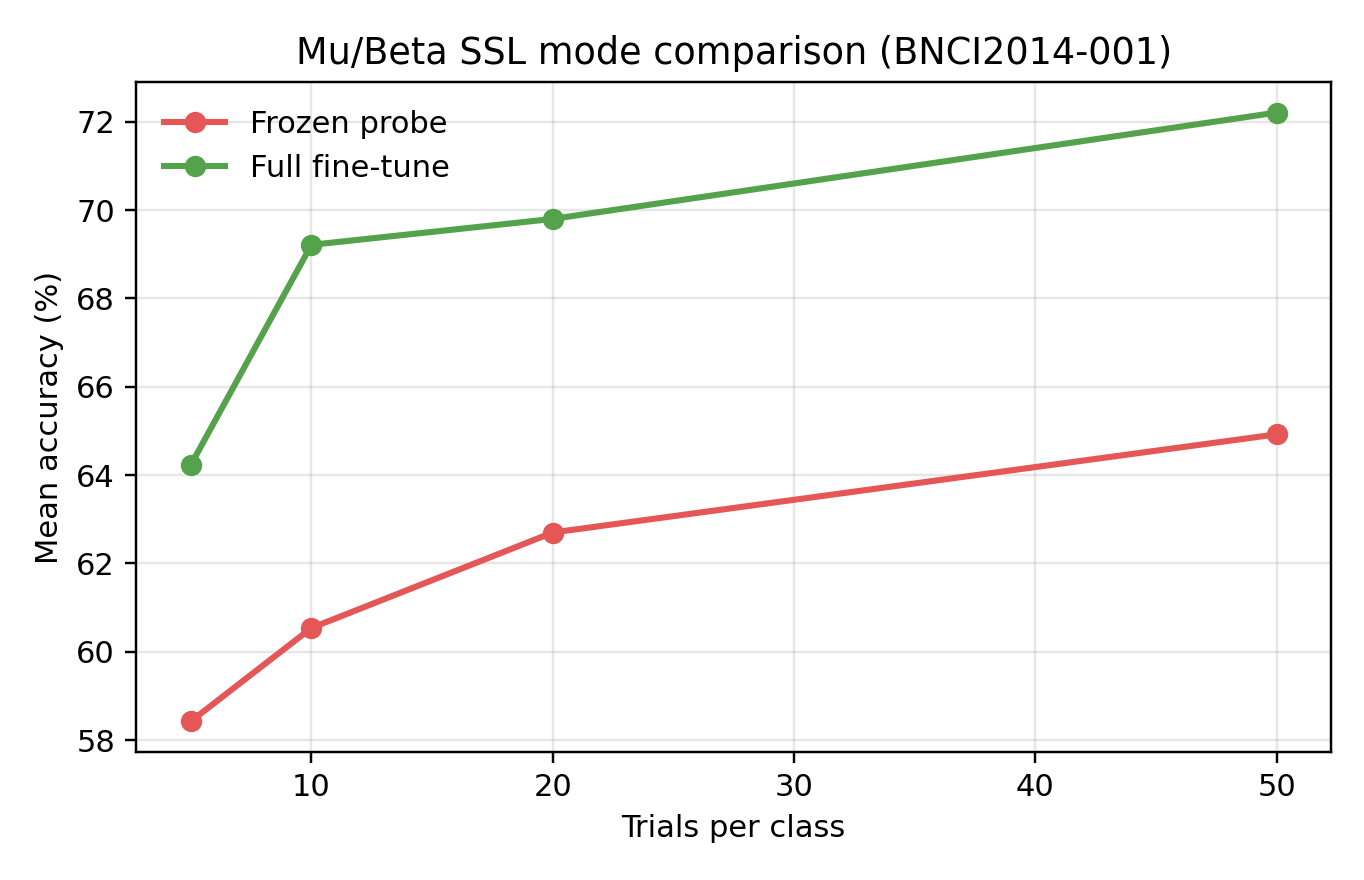
\includegraphics[width=0.88\textwidth]{figures/mu_beta_mode_comparison.png}
\caption{$\mu$/$\beta$ SSL mode comparison on BNCI2014-001 (frozen probe vs full fine-tune).}
\label{fig:mubeta_mode}
\end{figure}

\begin{figure}
\centering

\includegraphics[width=0.95\textwidth]{figures/physionetmi_per_subject_5shot.png}
\caption{PhysionetMI per-subject 5-shot results (subjects S1--S20, masked SSL full fine-tuning).}
\label{fig:physio_subject}
\end{figure}

\section{Discussion}

LoMI-SSL reveals three key insights for MI calibration:

\textbf{SSL $>$ deep-from-scratch.} Both masked reconstruction and physiology-aware SSL substantially outperform EEGNet-from-scratch (+13.7\% BNCI), validating representation learning for low-data regimes.

\textbf{CSP remains robust.} Classical CSP+LDA (58.8\%) matches/exceeds SSL on clean benchmarks, serving as critical baseline.

\textbf{Frozen probes fail universally.} All SSL methods require fine-tuning, highlighting projection head--encoder mismatch in EEG.

\textbf{Cross-dataset gaps are substantial.} BNCI$\rightarrow$PhysionetMI transfer degrades 7--10\%, reflecting montage/paradigm differences realistic for deployment.

\subsection{Deployment Readiness}

ONNX CPU inference: \SI{0.358}{\milli\second}/trial (batch=1). Peak VRAM during few-shot fine-tuning: $<$ \SI{500}{MB} (RTX 4050). int8 quantization drop: 23.6\% (room for QAT).

\begin{figure}
\centering

\includegraphics[width=0.75\textwidth]{figures/deployment_latency_vram.png}
\caption{Deployment metrics.}
\label{fig:deployment}
\end{figure}

\section{Limitations and Future Work}

Dataset scope (2 datasets) limits broad generalization claims. High per-subject variance ($\sigma=12.8\%$ PhysionetMI) reflects clinical realism but demands subject-independent methods. Future work: SNN conversion, larger multi-site corpora, real-time evaluation.

\ack{This work used publicly available MOABB datasets and open-source tooling from MOABB and Braindecode.}

\data{All datasets used are publicly available through MOABB. Aggregated result tables used in this manuscript are bundled in \texttt{paper/data}.}

\suppdata{Code and experiment scripts are available at \url{https://github.com/khresth/LoMI-SSL}.}

\section*{References}
\begin{thebibliography}{99}
\bibitem{lotte2018review}
Lotte R, Bougrain L, Cichocki A, Clerc M, Congedo M, Rakotomamonjy A and Yger F 2018 A review of classification algorithms for EEG-based brain-computer interfaces: a 10 year update \textit{J. Neural Eng.} \textbf{15} 031005

\bibitem{banville2021self}
Banville H, Chehab O, Hyvarinen A, Engemann D-A and Gramfort A 2021 Uncovering the structure of clinical EEG signals with self-supervised learning \textit{J. Neural Eng.} \textbf{18} 046020

\bibitem{tangermann2012benchmark}
Tangermann M, Muller K-R, Aertsen A, Birbaumer N, Braun C, Brunner C \textit{et al} 2012 Review of the BCI Competition IV datasets \textit{Front. Neurosci.} \textbf{6} 55

\bibitem{goldberger2000physiobank}
Goldberger A L, Amaral L A N, Glass L, Hausdorff J M, Ivanov P C, Mark R G, Mietus J E, Moody G B, Peng C-K and Stanley H E 2000 PhysioBank, PhysioToolkit, and PhysioNet: components of a new research resource for complex physiologic signals \textit{Circulation} \textbf{101} e215--e220

\bibitem{vandecappelle2022moabb}
Jayaram V and Barachant A 2018 MOABB: trustworthy algorithm benchmarking for BCIs \textit{J. Neural Eng.} \textbf{15} 066011

\bibitem{schirrmeister2025braindecode}
Gemein L A W, Schirrmeister R T and Braindecode contributors 2025 Braindecode: deep learning for EEG decoding (software) \url{https://braindecode.org}
\end{thebibliography}

\end{document}